\documentclass[main.tex]{subfiles}

\begin{document}

\section{Aufgabe 2}

Eine Fabrik stellt ein Gerät her, welches einen elektronischen Schalter enthält. Dieser Schalter wird von zwei Firmen A und B bezogen, wobei 60\% aller Schalter von A und 40\% aller Schalter von B stammen. Erfahrungsgemäß sind 5\% aller A-Schalter und 2\% aller B-Schalter defekt. Die Endkontrolle der Fabrik akzeptiert jeden intakten Schalter
und fälschlicherweise auch 5\% der defekten Schalter jeder Firma.
\begin{enumerate}
    \item Modellieren Sie die Situation durch ein geeignetes mehrstufiges Experiment und bestimmen Sie in diesem Modell die Wahrscheinlichkeit, dass ein Gerät in den Verkauf gelangt und einen defekten Schalter besitzt.
    \item Ein Kunde beanstandet einen gekauften Schalter. Wie wahrscheinlich ist es, dass der Schalter
    \begin{enumerate}
        \item von Firma A stammt?
        \item von Firma B stammt?
    \end{enumerate}
\end{enumerate}

\subsection{Lösung 2}
\begin{figure}[h]
    \makebox[\textwidth][c]{
        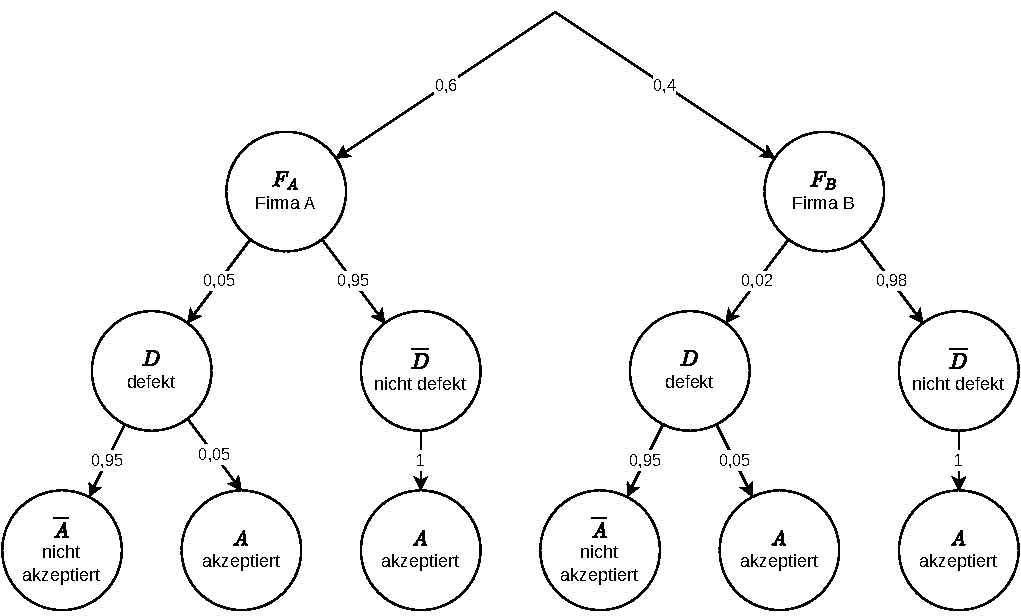
\includegraphics[width=1\linewidth]{A2.drawio.pdf}
    }
    \caption{Modell der Produktion und Prüfung}
    \label{fig:lgs2}
\end{figure}

\subsubsection{2a)}
Ein defektes Gerät gelingt in den Verkauf, wenn es defekt ist und fälschlicherweise durch die Endkontrolle akzeptiert wird. $P(A\cap D)$

$$\begin{aligned}
    P(A\cap D) &= P(F_A \cap D \cap A) + P(F_B \cap D \cap A) \\
    &= 0,6 \cdot 0,05 \cdot 0,05 + 0,4 \cdot 0,02 \cdot 0,05 \\
    &= 0,19 \%
\end{aligned}$$

\subsubsection{2b)}
Die Wahrscheinlichkeit, dass ein defekter, und in der Endkontolle akzeptierter, Schalter von
\begin{enumerate}
    \item[i.] Firma A stammt $P(F_A | A\cap D)$
    \item[ii.] Firma B stammt $P(F_B | B\cap D)$
\end{enumerate}
errechnet sich durch die Formel von Bayes:
$$
    P(B_i | A) = \frac{P(A\cap B_i)}{P(A)} = \frac{P(B_i) \cdot P(A|B_i)}{\sum \limits_{j\in I} P(A|B_j)\cdot P(B_j)}
$$

Das bedeutet hier: 
$$\begin{aligned}
    P(F_A | A\cap D) &= \frac{P(A\cap D \cap F_A)}{P(A\cap D)} \\[2mm]
    &= \frac{0,6 \cdot 0,05 \cdot 0,05}{0,0019} \\[2mm]
    &\approx 78,95 \% \\[4mm]
    P(F_B | A\cap D) &= \frac{P(A\cap D \cap F_B)}{P(A\cap D)} \\[2mm]
    &= \frac{0,4 \cdot 0,02 \cdot 0,05}{0,0019} \\[2mm]
    &\approx 21,05 \% \\
\end{aligned}$$


\end{document}
